\documentclass[doktyp=barbeit, sprache=german]{TUBAFarbeiten}
\usepackage[utf8]{inputenc}
\usepackage[T1]{fontenc}
\usepackage{graphicx} 
\usepackage{amsmath}
\usepackage{subcaption}
\usepackage{algorithm}
\usepackage{algorithmicx}
\usepackage[noend]{algpseudocode}
\usepackage[numbers]{natbib}

\newcommand*\rfrac[2]{{}^{#1}\!/_{#2}}

\captionsetup{compatibility=false}
\bibliographystyle{unsrt}
\TUBAFFakultaet{Fakultät für Mathematik und Informatik}
\TUBAFInstitut{Institut für Informatik}
\TUBAFLehrstuhl{Lehrstuhl für Künstliche Intelligenz und Datenbanken}
\TUBAFTitel{Eine Studie zur kombinatorischen Optimierung mit Ameisenalgorithmen}
\TUBAFBetreuer{Prof. Dr. H. Jasper}
\TUBAFKorrektor{M. Sc. V. Göhler}
\TUBAFAutor[S. Dressel]{Samuel Dressel}
\TUBAFStudiengang{Angewandte Informatik}
\TUBAFVertiefung{Künstliche Intelligenz}
\TUBAFMatrikel{59\,963}
\TUBAFDatum[2018-11-05]{05. November 2018}
\begin{document}
\maketitle
\tableofcontents
\newpage
\section{Einleitung}
\section{Grundlagen}
\subsection{Der Ameisenalgorithmus (Ant Colony Optimization)}
\subsubsection{Biologische Grundlagen}
Für das weitere Verständnis des \textit{Ameisenalgorithmus} (auch Ant Colony Optimization Algorithm oder kurz ACO) ist zunächst ein Blick auf die biologischen Grundlagen notwendig. Ein Tierstaat, wie er bei den Ameisen zu finden ist, funktioniert nur mit einer effektiven und sinnvollen Kommunikation. Methoden zur Verständigung wie das Kommunizieren über Vibrationen und Berührungen sind eher die Ausnahme und kommen nur in speziellen Situationen zum Tragen \cite{Ameisen}. Dagegen kommt zum größten Teil der Informationsaustausch über Duftstoffe (sog. Pheromone) zur Anwendung. Diese werden durch verschiedene Drüsen erzeugt und wiederum in unterschiedlicher Kombination und Konzentration abgegeben.
Diese Pheromone werden benutzt, um Nestgenossen zu erkennen oder um bei Gefahren Kampf- und Abwehrverhalten auszulösen. Hauptsächlich jedoch nutzen Ameisen die Pheromone um eine Duftspur über ihren Hinterleib abzugeben. Diese dient ihnen und dem restlichen Tierstaat als Orientierungshilfe. Zum einen werden damit Straßen zu anderen Kolonien gebildet - zum anderen dienen sie dazu, anderen Ameisen den Weg zu einer Nahrungsquelle zu zeigen. Die Tatsache, dass ein Weg mit einer höheren Pheromonkonzentration bevorzugt wird, ist Grundlagen des Ameisenalgorithmus.
\subsubsection{Der Ameisenalgorithmus}
Der historische Ursprung des Algorithmus findet sich in den Versuchen von Jean-Louis Deneubourg und seine Kollegen \cite{Biological}. Das sogenannte \glqq Double-Bridge-Experiment\grqq \,zeigte, dass Ameisen den kürzesten Weg aufgrund der Pheromonmarkierung finden. In diesem Experiment ist eine Kolonie von Argentinischen Ameisen mit einer Nahrungsquelle durch zwei Brücken verbunden, die gleichzeitig den einzigen Zugang zu dieser Nahrungsquelle bilden. \cite{Dorigo2007}. Dabei können die Ameisen die Futterquelle nur über diese zwei Brücken erreichen. Im ersten Teil des Versuchs sind diese beiden Brücken jeweils gleich lang (siehe Abbildung \ref{img:DBExperiment}a). Zu Beginn erkunden die Ameisen die Umgebung der Kolonie bis sie eine Entscheidung über die Auswahl der Brücke treffen müssen. Lässt sich aufgrund einer noch nicht stattgefundenen Begehung der Brücken keine Pheromonspur feststellen, so entscheiden die Ameisen rein zufällig welche Brücke sie wählen. Die Wahrscheinlichkeit für beide Wege liegt bei gleichen Bedingungen bei 50 Prozent. Wird der Versuch über längere Zeit durchgeführt, so wird durch Zufall die Pheromonkonzentration der einen Brücke höher sein als die der anderen. Diese wird dadurch attraktiver für die Ameisen und wird somit letztenendes der favorisierte Weg zur Nahrungsquelle. 
\\Im zweiten durchgeführten Versuch sind die beiden Brücken unterschiedlich lang (siehe Abbildung \ref{img:DBExperiment}b). Auch hier liegt die Wahrscheinlichkeit für beide Brücken zu Anfang bei 50 Prozent. Da die Ameisen, die sich für die kürzere Brücke entscheiden, schneller wieder zurück am Nest sind, steigt das Pheromonlevel auf diesem Weg deutlich schneller an. Nach einiger Zeit kristalliert sich die kürzere Brücke als optimale Route heraus, während der längere Weg durch eine natürliche Pheromonverdunstung immer unattraktiver wird. Im Vergleich zum ersten Versuch geschieht der Ausbau der Pheromonspur wesentlich schneller und effektiver.
\begin{figure}
\captionsetup[subfigure]{justification=centering}
\centering
\begin{subfigure}[c]{0.45\textwidth}
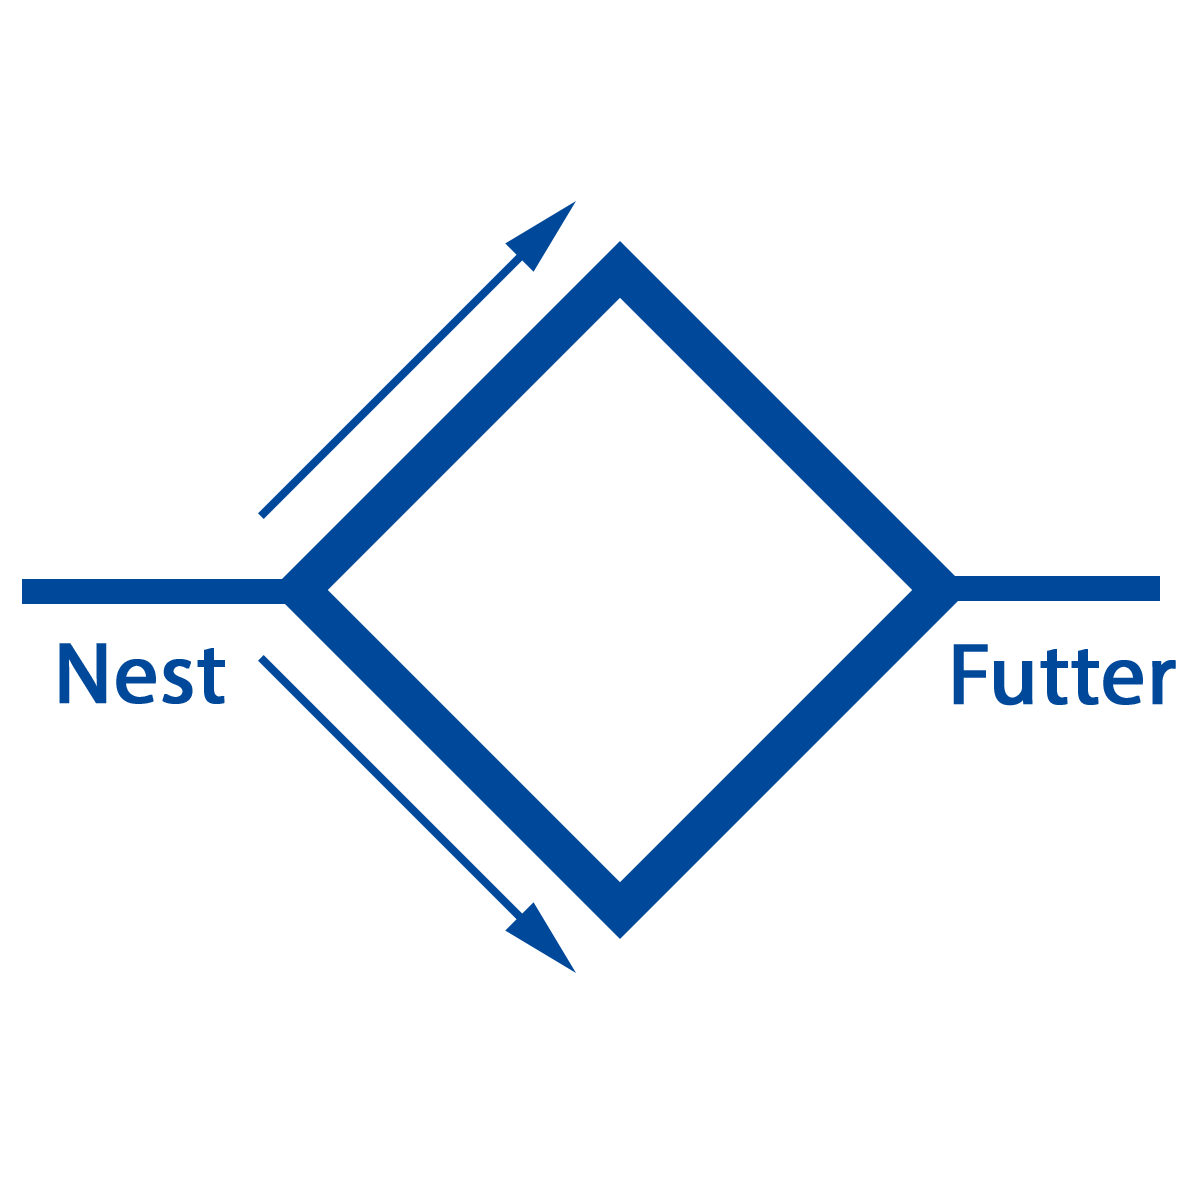
\includegraphics[width=0.9\textwidth]{images/RouteTrivial.png}
\subcaption{Skizze zu Versuch 1; beide Wege sind gleich lang}
\end{subfigure}
\begin{subfigure}[c]{0.45\textwidth}
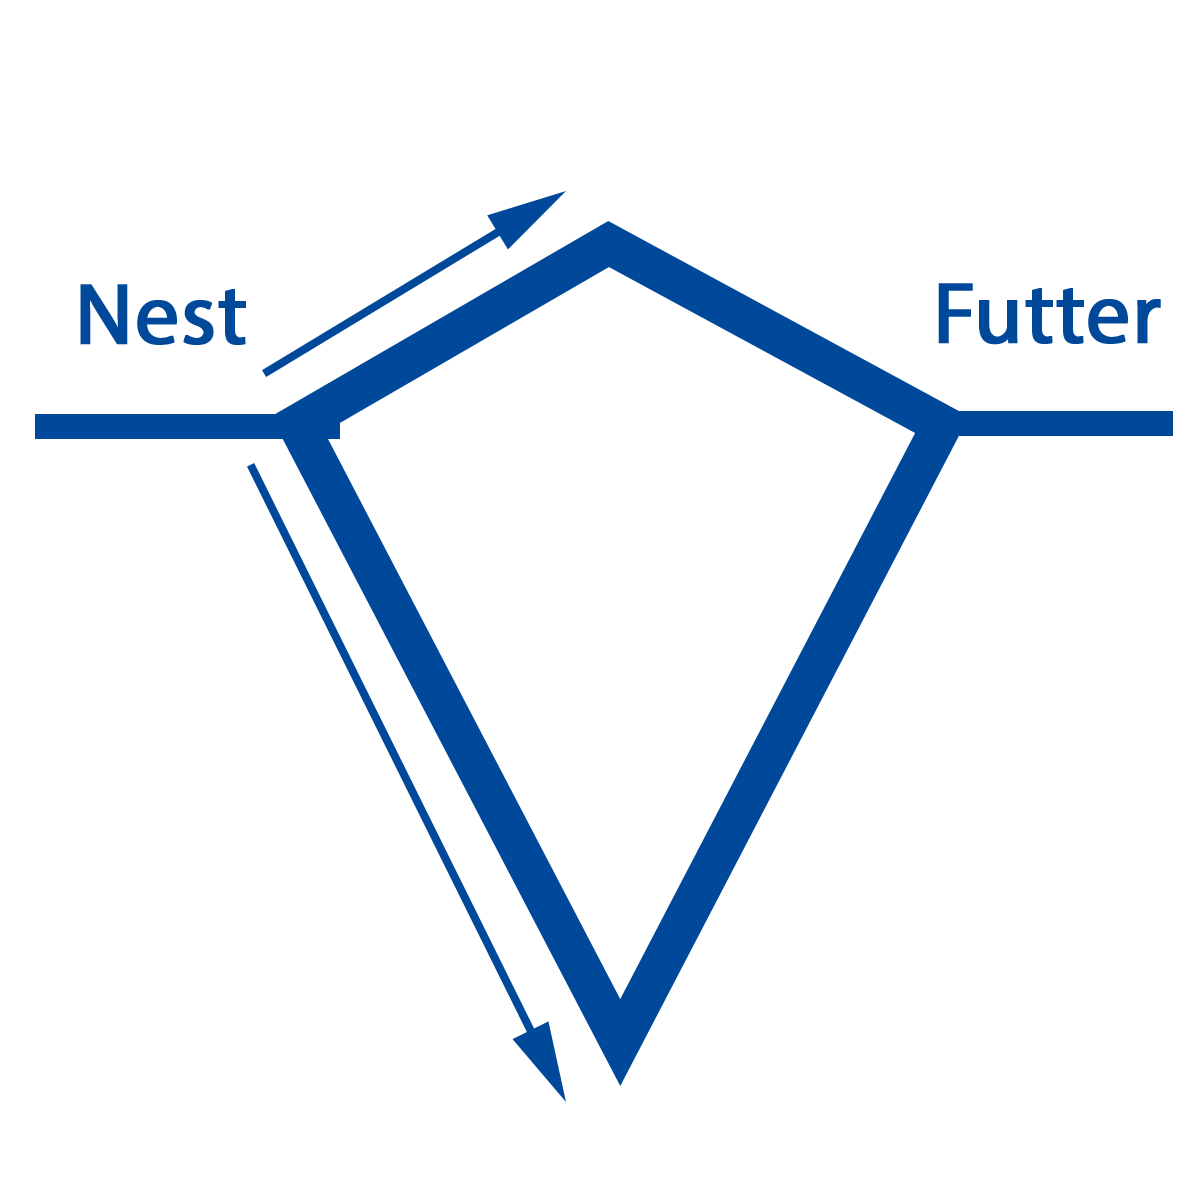
\includegraphics[width=0.9\textwidth]{images/RouteAdv.png}
\subcaption{Skizze zu Versuch 2; die Wege sind unterschiedlich lang}
\end{subfigure}
\caption{Double-Bridge-Experiment nach Deneubourg \cite{Biological}}
\label{img:DBExperiment}
\end{figure}
\subsection{Das Travelling-Salesman-Problem}
\subsubsection{Das Problem im Allgemeinen}
Das \textit{Travelling Salesman Problem} (im Folgenden mit TSP abgekürzt) ist eines der bekanntesten und meist untersuchten Optimierungsprobleme \cite{TaschenbuchAlgorithmen}. Kerninhalt des Problems ist dabei folgender: Ein Handlungsreisender soll in einer Rundreise \(n\) verschiedene Städte besuchen. Der Reisende startet dabei (zufällig) in einer dieser Städte und am Ende seiner Reise kehrt er auch wieder in diese Stadt zurück. Dabei sollen alle $n$ Städte nur einmal besucht werden und die Weglängen bzw. die Kosten der gesamten Reise minimal sein.
\\Seinen geschichtlichen Ursprung hat das TSP im Jahr 1832, als in Deutschland ein Buch mit dem Titel \glqq Der Handlungsreisende, wie er sein soll und was er zu thun hat, um Aufträge zu erhalten und eines glücklichen Erfolges in seinen Geschäften gewiss zu sein\grqq erschien. Dieses Buch und dessen Inhalt diente als Grundlage für die Erforschung des Problems. Die erste Benutzung des Ausdrucks \glqq Traveling Salesman Problem\grqq erfolgte in mathematischen Kreisen etwa um das Jahr 1931 \cite{TSP}. 
Dies geschah als mehrere amerikanische Mathematiker sich des Problems annahmen - wichtige Vertreter waren dabei Merrill Flood und Hassler Whitney, die die Überlegungen des österreichischen Mathematikers Karl Menger als Grundlage nahmen. Nach und nach wurde das Problem durch zahlreiche Veröffentlichungen immer präsenter und bis heute ist das TSP eines der prominentesten und am besten untersuchten Probleme in der Mathematik.
\subsubsection{Graphentheoretische Grundlagen} \label{graphbasics}
Um das Problem formal als ein graphentheoretisches Problem darzustellen, werden im Folgenden die dafür benötigten Begriffe definiert \cite{graphKemnitz}:
\\\\$G = (V,E,c)$ sei zunächst ein \textit{ungerichteter Graph}. Dabei beschreibt $V = \{1,...,n\}$ die Menge der Knoten und $E$ die Menge der Kanten, welche letztenendes eine Menge von ungeordneten Paaren $e \in E = \{i,j\}$ mit $i,j \in V$ ist. $c$ beschreibt die Gewichtung der einzelnen Kanten in $E$.
\\\\Ist $e = ij = \{i,j\}$ eine Kante von $G$, dann verbindet $e$ die Knoten $i$ und $j$. Diese Knoten $i,j$ heißen dann \textit{adjazent}. Die Kante $e$ dagegen heißt dann \textit{inzident} zu $i$ und $j$. 
\\\\Die Menge $N(v)$ aller Knoten von $G$, die zu $v$ adjazent sind, nennt man \textit{Nachbarschaft} von $v$.
\\\\Ein weiterer wichtiger Begriff ist der \textit{Grad} $d$ eines Knotens $v \in V$. Dabei ist der Grad $d(v)$ die Anzahl der zu $v$ inzidenten Kanten.
\\\\Eine \textit{Kantenfolge} $W = (v_0v_1,v_1v_2,...,v_{r-1}v_r)$ eines Graphen $G$ ist eine Folge von Kanten. Wenn alle Kanten in dieser Kantenfolge verschieden sind, dann heißt diese Folge \textit{Kantenzug}. Sind zudem noch alle Knoten paarweise verschieden, so erhält man einen \textit{Weg} $P$.
\\\\Gilt $v_0 = v_r$, so heißt der Weg geschlossen oder auch \textit{Kreis}.
\\\\Enhält so ein Kreis $C$ nicht unbedingt jede Kante $e$ von $G$, aber dafür jeden Knoten $v$ von $G$ genau einmal, so nennt man diesen Kreis einen \textit{Hamiltonkreis} $\pi$ (auch \textit{Tour}) von $G$ \cite{graphDiestel}. Ein Hamiltonkreis $\pi$ heißt dann \textit{optimal}, wenn die Summe der Kantengewichte minimal wird.
\\\\Existiert in $G$ ein Kantenzug $Z$, der alle Kanten enthält und zudem geschlossen ist, dann heißt $Z$ \textit{Eulertour} und $G$ \textit{eulerscher Graph} \cite{graphKemnitz}.
\\\\Für die Betrachtung von möglichen Lösungsalgorithmen des TSP müssen nun noch abschließend der Begriff des Baums und des Matchings definiert werden:
\\Ein \textit{Baum} ist ein zusammenhängender, kreisloser Graph. Ein Baum $T$ heißt \textit{Spannbaum} von $G$, wenn er $G$ ganz aufspannt, d.h. wenn $V(T) = V(G)$ ist. Der Spannbaum ist \textit{minimal}, wenn seine Länge minimal ist.
\\\\$M$ ist ein \textit{Matching} von $U \subseteq V$, wenn jeder Knoten $U$ mit einer Kante aus $M$ inzidiert.
\\\\Auf dieser mathematischen Grundlage lässt sich das TSP nun wie folgt definieren: 
\\$G = (V,E,c)$ sei Graph und $F$ die Menge aller Hamiltonkreise in $G$. Ziel ist nun das Finden des Hamiltonkreises $f \in F$, für den die Summe der einzelnen Kantenkosten minimal wird \cite{TSPVariations}.
\\\\Unter der bislang unbewiesenen Annahme, dass die Komplexitätsklassen $P$ und $NP$ verschieden sind, gehört das TSP zur Klasse der NP-vollständigen Probleme, was bedeutet dass es sich nicht mit einem deterministischen Algorithmus in Polynomialzeit lösen lässt \cite{Applegate2007}.  Alle ansatzweise effektiven Möglichkeiten und Algorithmen zur Lösung von TSP-Instanzen mit sehr vielen Städten basieren deshalb auf heuristischen Verfahren. Für Probleme mit weniger Städten gibt effektive Direktlöser, die das optimale Ergebnis in durchaus annehmbarer Zeit liefern.
\subsubsection{Ansätze und Algorithmen zur Lösung des Problems}
Da das Problem wie oben schon erwähnt zu den NP-vollständigen Problemen gehört, ist ein Algorithmus zur Lösung des TSP schnell oder er findet eine optimale Tour - aber er wird nicht beide Eigenschaften besitzen \cite{TSP}. Deswegen unterscheidet man wie auch allgemein bei anderen kombinatorischen Optimierungsproblemen zwischen exakten und heuristischen Algorithmen.
Der einfachste Algorithmus zur exakten Lösung des TSP ist die sogenannte \textit{"brute-force\grqq} \, oder naive Methode \cite{TaschenbuchAlgorithmen}. Dieser Algorithmus betrachtet nacheinander alle möglichen Touren und deren Länge und ermittelt durch den Vergleich derselben die optimale und kürzeste Tour. 
Ist der Graph \(G\), der dieses Problem modelliert, ein ungerichteter Graph, so muss man mit diesem Algorithmus \(\frac{1}{2} \cdot (n - 1)!\) verschiedene Rundreisen betrachten. Bei neun verschiedenen Städten ergeben sich daraus 20160 verschiedene Touren, bei 16 Städten dagegen schon ca. 653 Milliarden Routen, dies macht Algorithmus für die meisten Optimierungsprobleme völlig unbrauchbar. Auch andere exakte Methoden haben oft einen hohen Rechen- und Zeitaufwand. Man entscheidet sich deswegen häufig dafür effiziente heuristische Algorithmen zu konstruieren, die zwar nicht immer eine optimale Tour finden, aber zumindest eine nahezu optimale Tour. Es existiert eine Vielzahl solch heuristischer Verfahren Eines der intuitivsten ist der \textit{Nearest-Neighbor-Algorithmus} \cite{Lotz2014}. Hierbei wird ein zufälliger Knoten $v_1$ als Startknoten ausgewählt. Danach wird iterativ immer der Knoten $v_i$ ausgewählt, der dem zuletzt ausgewählten Knoten am nächsten liegt und noch nicht in der schon besuchten Knotenmenge $V^\prime$ enthalten ist. Der Algorithmus ist beendet, wenn alle Knoten besucht wurden. Das Problem hierbei ist, dass die letzte Kante, die den letzten Knoten mit dem Startknoten verbindet und den Hamiltonkreis vervollständigt, eine mehr oder weniger beliebige Länge haben kann und somit die Bestmöglichkeit der gefundenen Lösung wesentlich einschränkt. Formal lässt sich der Algorithmus wie folgt darstellen: 
\begin{algorithm}
\caption{Nearest-Neighbor-Algorithm}
\label{euclid}
\textbf{Eingabe:} $G = (V,E,c)$
\\\textbf{Ausgabe:} Tour $\pi$, die alle Knoten $v \in V$ besucht
\begin{algorithmic}[1]
\State $z_1 := v \in V$
\State $V^\prime := V \, \backslash \, \{v_1\}$
\State $i := 2$
\While {$V^\prime \ne \emptyset$}
\State $z_1 := min_{v\in V^\prime}  \, c(\{v_{i-1},v\})$
\State $V^\prime := V^\prime \, \backslash \, \{v_i\}$
\State $i := i +1 $
\EndWhile
\State $\pi := (v_1,...,v_n,v_1)$
\end{algorithmic}
\end{algorithm}
\\Ein weiterer bekannter heuristischer Algorithmus ist die \textit{Minimal-Spaaning-Tree-Heuristik, kurz MST}. Dabei wird zunächst ein minimaler Spannbaum $T$ für den Graphen $G$ ermittelt \cite{Groetschel2005}. Zur Ermittlung dieses minimalen Spannbaumes stehen mehrere Algorithmen zur Verfügung (Algorithmus von Prim, Algorithmus von Kruskal, ...) \cite{MST}. 
\begin{algorithm}
\caption{Algorithmus von Prim}
\label{prim}
\textbf{Eingabe:} $G = (V,E,c)$
\\\textbf{Ausgabe:} Minimaler Spannbaum T
\begin{algorithmic}[1]
\State $T := \emptyset$
\State $r := v \in V$
\State $U := \{r\}$
\While {|U| < |V|}
\State Finde $u \in U$ und $v \in V - U$ mit $(u,v)$ ist minimal
\State $T := T + \{(u,v)\}$
\State $U := U + \{v\}$
\EndWhile
\end{algorithmic}
\end{algorithm}
\\Danach wird jede Kante innerhalb des Spannbaumes verdoppelt; es entsteht der eulersche Graph $G^\prime$. Nun wählt man einen beliebigen Startknoten und folgt den Kanten im Sinne einer Eulertour. Bereits besuchte Kanten werden dabei gestrichen und stattdessen die direkte Verbindung zwischen den jeweils verbleibenden Knoten gewählt. Das \textit{Verfahren von Christofides} baut auf diesem Algorithmus und erweitert diesen dadurch, dass der minimale Spannbaum nicht verdoppelt wird, sondern das minimale Matching von den Knoten in $B$ sucht, die einen ungeraden Grad haben. Nach der Dreiecksungleichung gilt, dass die Summe der Längen zweier Seiten $a$ und $b$ stets mindestens so groß ist wie die Länge der dritten Seite (formal: $c \leq a + b$). Die MST-Heuristik ist deswegen höchstens doppelt so lang, die Christofides-Heuristik höchstens höchstens 1,5-mal so lang wie die optimale Lösung \cite{Groetschel2005}.
\subsubsection{TSPLIB als Quelle für bekannte Probleme} \label{TSPLIB}
Die in dieser Arbeit untersuchten Probleminstanzen stammen aus der TSPLIB der Universität Heidelberg. Bekannte Probleme wurden dort in ein einheitliches Datenformat gebracht und eignen sich deswegen gut zur Auswertung von Implementierungen des TSP. Die Daten werden als XML-Datei (Extensible Markup-Language-File) angeboten, was die Anwendung der Lösungsalgorithmik auf viele verschiedene Probleme vereinfacht. \cite{TSPLIB}.
\subsubsection{Möglichkeiten der Distanzberechnung}
Um das TSP lösen zu können, benötigt man Informationen über die Distanzen bzw. die Wegkosten zwischen den einzelnen Knoten. In der TSPLIB (siehe \ref{TSPLIB}) sind dabei die Kantenwerte schon berechnet worden. Dieser Berechnung hängt vom Format der Positionsinformationen der einzelnen Knoten ab. Die zwei wichtigsten Distanzarten, die auch den Daten in dieser Arbeit zu grunde liegen, sind die \textit{Euklidische Distanz} und die \textit{Geographische Distanz}. Die Euklidische Distanz (auch euklidischer Abstand) ist der triviale Abstand zwischen zwei Punkten den man auch durch Messung mit einem einfachem Längenmessgerät wie einem Lineal ermittelt \cite{Distanz}. Die Distanz $d_{xy}$ der Punkte $x$ und $y$ in einer Ebene mit den Koordinaten $x = (x_1, x_2)$ und $y = (y_1, y_2)$ ergibt sich dabei aus folgender Formel:
\begin{align}
\label{eq:Euclid}
d_{xy} = \left\| x - y \right\|_2 = \sqrt{{(y_1-x_1)}^2+{(y_2-x_2)}^2}
\end{align}
Die Ermittlung der geographischen Distanz ist dagegen etwas komplizierter. Dies hat die Ursache, dass die Koordinaten auf einer annähernd idealen Kugel liegen. Betrachtet man die Erde als ideale Kugel mit einem Radius $r = 6378,388 \,km$ und liegen die Koordinaten in der Dezimalschreibweise (beispielsweise $Lat=45.345^\circ$, $Long=-3.234^\circ$) vor, ergibt sich für die für zwei Städte $i$ und $j$ folgende Berechnung:
\begin{algorithm}
\caption{Geographische Distanz}
\label{geodistance}
\begin{algorithmic}[1]
\State $r = 6378,388$
\State $latitude_i = latitude_i \cdot \pi / 180; \,latitude_j = latitude_j \cdot \pi / 180$
\State $longitude_i = longitude_i \cdot \pi / 180;\, longitude_j =longitude_j \cdot \pi / 180$
\State $q_1 = cos(longitude_i - longitude_j)$
\State $q_2 = cos(latitude_i - latitude_j)$
\State $q_3 = cos(latitude_i + latitude_j)$
\State \textbf{$d_{ij} = r * arccos(0,5 \cdot ((1 + q_1) \cdot q_2 - (1 - q_1) \cdot q_3)) + 1)$}
\end{algorithmic}
\end{algorithm}
\subsection{Das Travelling-Salesman-Problem und der Ameisenalgorithmus}
Betrachtet man den Ameisenalgorithmus, so ähnelt dies dem TSP sehr stark. Dies war auch der Grund, warum der Ameisenalgorithmus zuerst als Lösung in Form des \textit{Ant-Systems (AS)} für das TSP zur Anwendung kam \cite{MaxMin}.
\\Es bietet sich an, dass TSP wie in Abschnitt \ref{graphbasics} schon näher erläutert als Graphenproblem zu modellieren:
Hat man ein TSP mit $n$ Städten, so benötig man neben einer $n\times n$-Matrix $D$ mit den verschiedenen Distanzen zwischen den Knoten auch eine $n\times n$-Matrix $T$ mit den verschiedenen Pheromonkonzentrationen. Dabei ist das Element $\tau_{ij}$ die Pheromonkonzentration auf der Kante zwischen Knoten $i$ und $j$, analog ist die Distanz $d_{ij}$ die Distanz zwischen den Knoten $i$ und $j$. Ist das verwendete TSP symmetrisch, dann ist auch die Pheromonspur symmetrisch; das heißt: $\tau_{ij} = \tau_{ji}$.
Abstrakt gesehen werden dann zunächst alle $m$ Ameisen einer Menge $M$ auf verschiedene zufällig gewählte Knoten gesetzt. Danach bewegt sich jede Ameise $m_k$ in jedem darauffolgenden Iterationsschritt zu einem weiteren Knoten, falls sie diesen vorher noch nicht besucht hat und insgesamt nicht alle Knoten schon besucht wurden. 
\\\\Der Entscheidung, welcher Knoten als nächstes besucht wird, liegen gewisse Regeln zugrunde. Zum einen hat die Pheromonkonzentration der jeweiligen Kanten zu den anderen Knoten Einfluss auf die Entscheidung, zum anderen die heuristische Information $\eta_{ij}$. Die heuristische Information ergibt sich dabei aus der Distanz:
\begin{align}
\label{eq:Heuristic}
\eta_{ij} = \rfrac{1}{d_{ij}}
\end{align}
Bei der Wahl des nächsten Knotens bevorzugen die Ameisen solche Knoten, die relativ nah gelegen sind und die durch eine Kante mit hoher Pheromonkonzentration verbunden sind.
Die Wahrscheinlichkeit $p^k_{ij}$, mit der eine Ameise $k \in M$ ausgehend von eines Knotens $i$ den nächsten Knoten $j$ besucht, kann durch die Gleichung \ref{eq:Prob} ausgedrückt werden.
Dabei sind $\alpha$ und $\beta$ Parameter, die im Fall von $\alpha$ die Wichtigkeit der Pheromonkonzentration und im Fall von $\beta$ die Wichtigkeit der Distanzinformationen zur Entscheidungsfindung angeben. $N^k_i$ ist die Menge der erreichbaren unbesuchten Knoten der Ameise $m_k$.
\begin{align}
\label{eq:Prob}
p^k_{ij} = \frac{[\tau_{ij}]^\alpha \, [\eta_{ij}]^\beta}{\sum\nolimits_{l\in N^k_i} [\tau_{il}]^\alpha \, [\eta_{il}]^\beta} \; \; \text{if}\: j \in N^k_i
\end{align}
Jede Ameise merkt sich zudem die Reihenfolge der besuchten Knoten in einer Liste $L$. Falls eine Ameise $m_k$ alle Knoten $n$ besucht hat, kehrt sie zu ihrem Anfangsknoten zurück und beendet ihre Tour. Anhand der Liste mit den besuchten Knoten lässt sich nun ein valider Hamiltonkreis ableiten. 
\\Außerdem ist diese Liste notwendig, um die Pheromonkonzentration der benutzten Kanten zu aktualisieren.
\\Für ein Pheromonupdate gibt es verschiedene Möglichkeiten, die für 2., 3. und 4. im Rahmen dieser Bachelorarbeit auch umgesetzt wurden: 
\begin{enumerate}
\label{enum:Update}
\item Aktualisierung der Pheromonkonzentration nachdem alle Ameisen $m \in M$ ihre Tour beendet haben
\item Aktualisierung der Pheromonkonzentration iterativ nach der erfolgreichen Tourkonstruktion jeder einzelnen Ameise $m_k$
\item Aktualisierung der Pheromonkonzentration nur durch die Ameise $m_k$, welche nach Beendigung der Tour die kürzeste Tour gefunden hat
\item Aktualisierung der Pheromonkonzentration für alle Ameisen $m \in M$ parallel, nachdem der jeweils nächste Knoten erreicht wurde
\end{enumerate}
Die Berechnung der neuen Pheromonkonzentration $\tau_{ij}$ zum Zeitpunkt $t + 1$ ist für alle Varianten gleich. Eine wichtige Variable, die hierauf Einfluss hat, ist zum einen $\Delta \tau^k_{ij}(t)$. Diese stellt dabei die Menge an Pheromon dar, die eine Ameise $k$ auf der jeweilige Kante $\{i,j\}$ ablegt. Zum anderen ist das der Parameter $\rho$, der für $1-\rho$ die verdunstende Menge an Pheromon angibt. Dieser Verdunstungsmechanismus hilft über die Zeiten ungünstige Kanten zu \glqq vergessen\grqq. Letztendlich berechnet sich die neue Pheromonkonzentration wie folgt:
\begin{align}
\label{eq:Pheromone}
\tau_{ij}(t+1) = \rho \, \tau_{ij}(t) + \sum_{k=1}^m \Delta \tau^k_{ij}(t)
\end{align}
\section{Implementierung des Problems in C++}
\subsection{Programmstruktur und Funktionsweise}
Das Programm lässt sich grob gesehen in zwei Komponenten aufteilen - zum einen in eine $C++$ Anwendung auf Konsolenbasis, welche den Algorithmus an sich ausführt. Die andere Kompononente ist ein in $C++/CLI$ umgesetzte einfache GUI. Wesentlich für das Verständnis der Implementierung ist lediglich die Programmstruktur und der Code der nativen $C++$-Konsolenanwendung. 
\begin{figure}
\captionsetup{justification=centering}
  \centering
     \includegraphics[width=0.9\textwidth]{images/classdiagram.png}
  \caption{Klassendiagramm zur Umsetzung des C++-Algorithmus mit den wesentlichen Attributen und Methoden}
  \label{img:classdiagram}
\end{figure}
\\\\Wie auch in Abbildung \ref{img:classdiagram} ersichtlich ist, besteht das Programm aus vier verschiedenen Klassen. Von grundlegender Bedeutung ist hierbei die Klasse \texttt{Ant}. Diese stellt die einzelnen Ameisen mit allen wichtigen Parametern und Methoden zur Wegfindung und Routenfindung dar. Jedes dieser \texttt{Ant}-Objekte greift auf eine gemeinsames Datenelement \texttt{XMLData} zu, in welchem die Daten der Städte sowie die Kosten- und Pheromonwerte zwischen den einzelnen Städten gespeichert sind. Beim Ausführen des Programms wird dieses Datenelement angelegt und initialisiert. Hierfür wird dem Konstruktor der Dateipfad zu einer Probleminstanz aus der TSPLIB (siehe Abschnitt \ref{TSPLIB}) übergeben und die dort enthaltenen Daten ausgelesen. Die Daten der Städte werden in einen Container aus \texttt{City}-Objekten gespeichert. Ein solches \texttt{City}-Objekt besteht aus dem Namen der Stadt und den Koordinaten und liefert gleichzeitig die Methode \texttt{measureDistance} zur Berechnung der Distanz zwischen zwei Städten. Im Falle der TSPLIB ist die Distanzberechnung aber überflüssig, da die Distanzwerte in der XML-Datei enthalten sind. Bei Anlage eines \texttt{XMLData}-Objekts werden diese Distanzwerte in einer Distanzmatrix abgespeichert sowie eine Matrix für die Pheromonwerte initialisiert. 
\\Desweiteren besitzt die Klasse \texttt{Ant} ein Memberobjekt der Klasse \texttt{Route}, in der die Abfolge der besuchten Städte gespeichert wird. 
\\\\Beim Start des Programms ein dynamischer Container vom Typ \texttt{vector<Ant>} angelegt, in dem sich alle \texttt{Ant}-Objekte befinden. Die weitere Arbeitsweise des Programms hängt nun von dem ausgewählten Algorithmus ab. Wie schon im obigen Abschnitt \ref{enum:Update} vorgestellt, unterscheiden sich die verschiedenen Algorithmen durch die Art und Weise der Aktualisierung der Pheromonkonzentration auf den einzelnen Kanten.
\\\\Bei der ersten implementierten Methode wird die Pheromonaktualisierung iterativ nach jeder erfolgreichen Tourkonstruktion einer Ameise vorgenommen. Der Algorithmus endet dann, wenn alle Ameisen ihre Tour beendet haben oder wenn nach einer bestimmten Anzahl von Iterationen keine kürzere Route mehr gefunden wurde.
\begin{algorithm}
\caption{Iterative Tourkonstruktion}
\label{IterativeTour}
\textbf{Eingabe:} Datenobjekt mit $v$ Städten sowie einer Distanzmatrix $D$ und Pheromonmatrix $S$, \texttt{vector} $M$ mit $m$ Ameisen, Iterationsschwelle $n$
\\\textbf{Ausgabe:} Route $r$ mit der kürzesten gefunden Distanz $d_s$
\begin{algorithmic}[1]
\State $i := 1$ (derzeitige Iteration nachdem das letzte Mal eine kürzere Route gefunden wurde)
\State $d_s := \infty$ (kürzeste gefunden Routenlänge)
\For{\textbf{each} Ameise $m_i \in M$}
\If {$i \leq n$}
\State $b_m := 1$ (Anzahl der besuchten Städte)
\State $d_m := 0$ (Routenlänge der Ameise $m_i$)
\State Starte in einer zufälligen Stadt $v_0$
\While{$b \neq v$}
\State Ermittle die nächste Stadt $v_i$ und gehe dorthin
\State $r_{m_i} := v_i$
\State $d_m := d_m + D_{i-1,i}$
\State $b_m := b_m + 1$
\EndWhile
\If{$d_m \leq d_s$}
\State $d_s := d_m$
\State $i := 1$
\EndIf
\State Aktualisiere Pheromonmatrix $S$
\State $i := i + 1$
\EndIf
\EndFor
\end{algorithmic}
\end{algorithm}
\\Die zweite implementierte Methode ist der ersten sehr ähnlich. Auch hier konstruieren alle Ameisen nacheinander ihre Tour. Jedoch wird die Pheromonmatrix nur durch die Ameise aktualisiert, welche die kürzeste Route gefunden hat. Diese Vorgehensweise basiert auf dem \textit{Max-Min-Ant-System} von Thomas Stüzle und Holger H. Hoos \cite{MaxMin}. Die iterative Tourkonstruktion erfolgt bei diesem Algorithmus notwendigerweise mehrmals. 
\\Bei der dritten in dieser Arbeit betrachteteten Methode konstruieren die Ameisen ihre Route parallel. Nach jeder erreichten Stadt wird die Pheromonkonzentration der letzten bereisten Kante aktualisiert. Wenn jede Ameise jede Stadt einmal besucht hat, endet der Algorithmus. Die kürzeste Route ergibt sich nun durch den Vergleich der Routenlänge aller Ameisen.
\begin{algorithm}
\caption{Parallele Tourkonstruktion}
\label{ParallelTour}
\textbf{Eingabe:} Datenobjekt mit $v$ Städten sowie einer Distanzmatrix $D$ und Pheromonmatrix $S$, \texttt{vector} $M$ mit $m$ Ameisen
\\\textbf{Ausgabe:} Route $r$ mit der kürzesten gefunden Distanz $d_s$
\begin{algorithmic}[1]
\State $j := 0$
\While{$j < v$}
\For{\textbf{each} Ameise $m_i \in M$}
\State Ermittle die nächste Stadt $v_i$ und gehe dorthin
\State $r_{m_i} := v_i$
\State $d_m := d_m + D_{i-1,i}$
\State Aktualisiere Pheromonmatrix $S$
\EndFor
\State $j := j + 1$
\EndWhile
\State $d_s = \infty$
\For{\textbf{each} Ameise $m_i \in M$}
\If{Tourlänge $d_m < d_s$}
\State $d_s := d_m$
\EndIf
\EndFor
\end{algorithmic}
\end{algorithm}
\subsection{Vorgehensweise zur Untersuchung von verschiedenen Datensätzen mit verschiedenen Implementierungen}
\section{Ergebnisse der Durchführung}
\subsection{Resultate bei Iteration einzelner Ameisen nacheinander}
\subsection{Resultate bei paralleler Erschließung}
\section{Auswertung und Vergleich}
\subsection{Vergleich der iterativen und parallelen Implementierung}
\subsection{Vergleich mit der optimalen Lösung}
\subsection{Vergleich mit der Laufzeit und Komplexität von anderen Algorithmen}
\section{Zusammenfassung und Fazit}
\newpage
\appendix
\section{Anhang}

\newpage
\bibliography{literatur}{}
\addcontentsline{toc}{section}{Literatur} 
\end{document}